% Qualitative: inline-math splicing (v19 -> v20), REAL benchmark example.
% Page page-cc37a835-... (EN academic literature). GT annotates the inline chips
% as $ {I}_{11} $ / $ {I}_{12} $. v19 OCR read them as the digit strings 111/112
% (unmatched by the harness); v20 recognizes the chips and splices them back as
% inline LaTeX, rendered/paired exactly like the ground truth. Input crop:
% fig/splice_input.png (region [160,372,905,431] of the page image).
\begin{tikzpicture}[font=\footnotesize]
  \node[inner sep=0pt] (in) at (0,1.45) {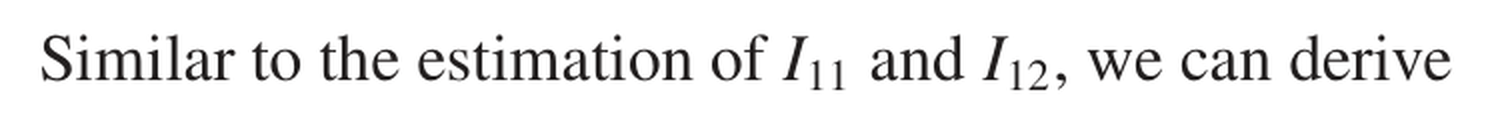
\includegraphics[width=8.2cm]{fig/splice_input}};
  \node[anchor=west, font=\tiny\itshape, text=black!55] at (in.north west)
        {input region (benchmark page)};
  \node[anchor=north, text width=3.7cm, draw=red!45, fill=red!4, rounded corners,
        inner sep=4pt] (bef) at (-2.15,0.7)
    {\textbf{v19}~{\scriptsize\itshape garble, unmatched}\\[3pt]
     \normalfont\ttfamily\small \dots of {\color{red!75!black}\textbf{111}} and
     {\color{red!75!black}\textbf{112}}, we can derive};
  \node[anchor=north, text width=3.7cm, draw=green!50!black, fill=green!6,
        rounded corners, inner sep=4pt] (aft) at (2.15,0.7)
    {\textbf{v20}~{\scriptsize\itshape spliced \LaTeX{}, matches GT}\\[3pt]
     \normalfont\small \dots of {\color{green!45!black}$I_{11}$} and
     {\color{green!45!black}$I_{12}$}, we can derive};
\end{tikzpicture}
